\documentclass[border=10pt]{standalone}
\usepackage[svgnames]{xcolor}
\usepackage{amsmath}
\usepackage{pgfplots}
\pgfplotsset{compat=newest}
\usepackage[sfdefault]{FiraSans}
\usepackage{FiraMono}
\renewcommand*\familydefault{\sfdefault}
\begin{document}
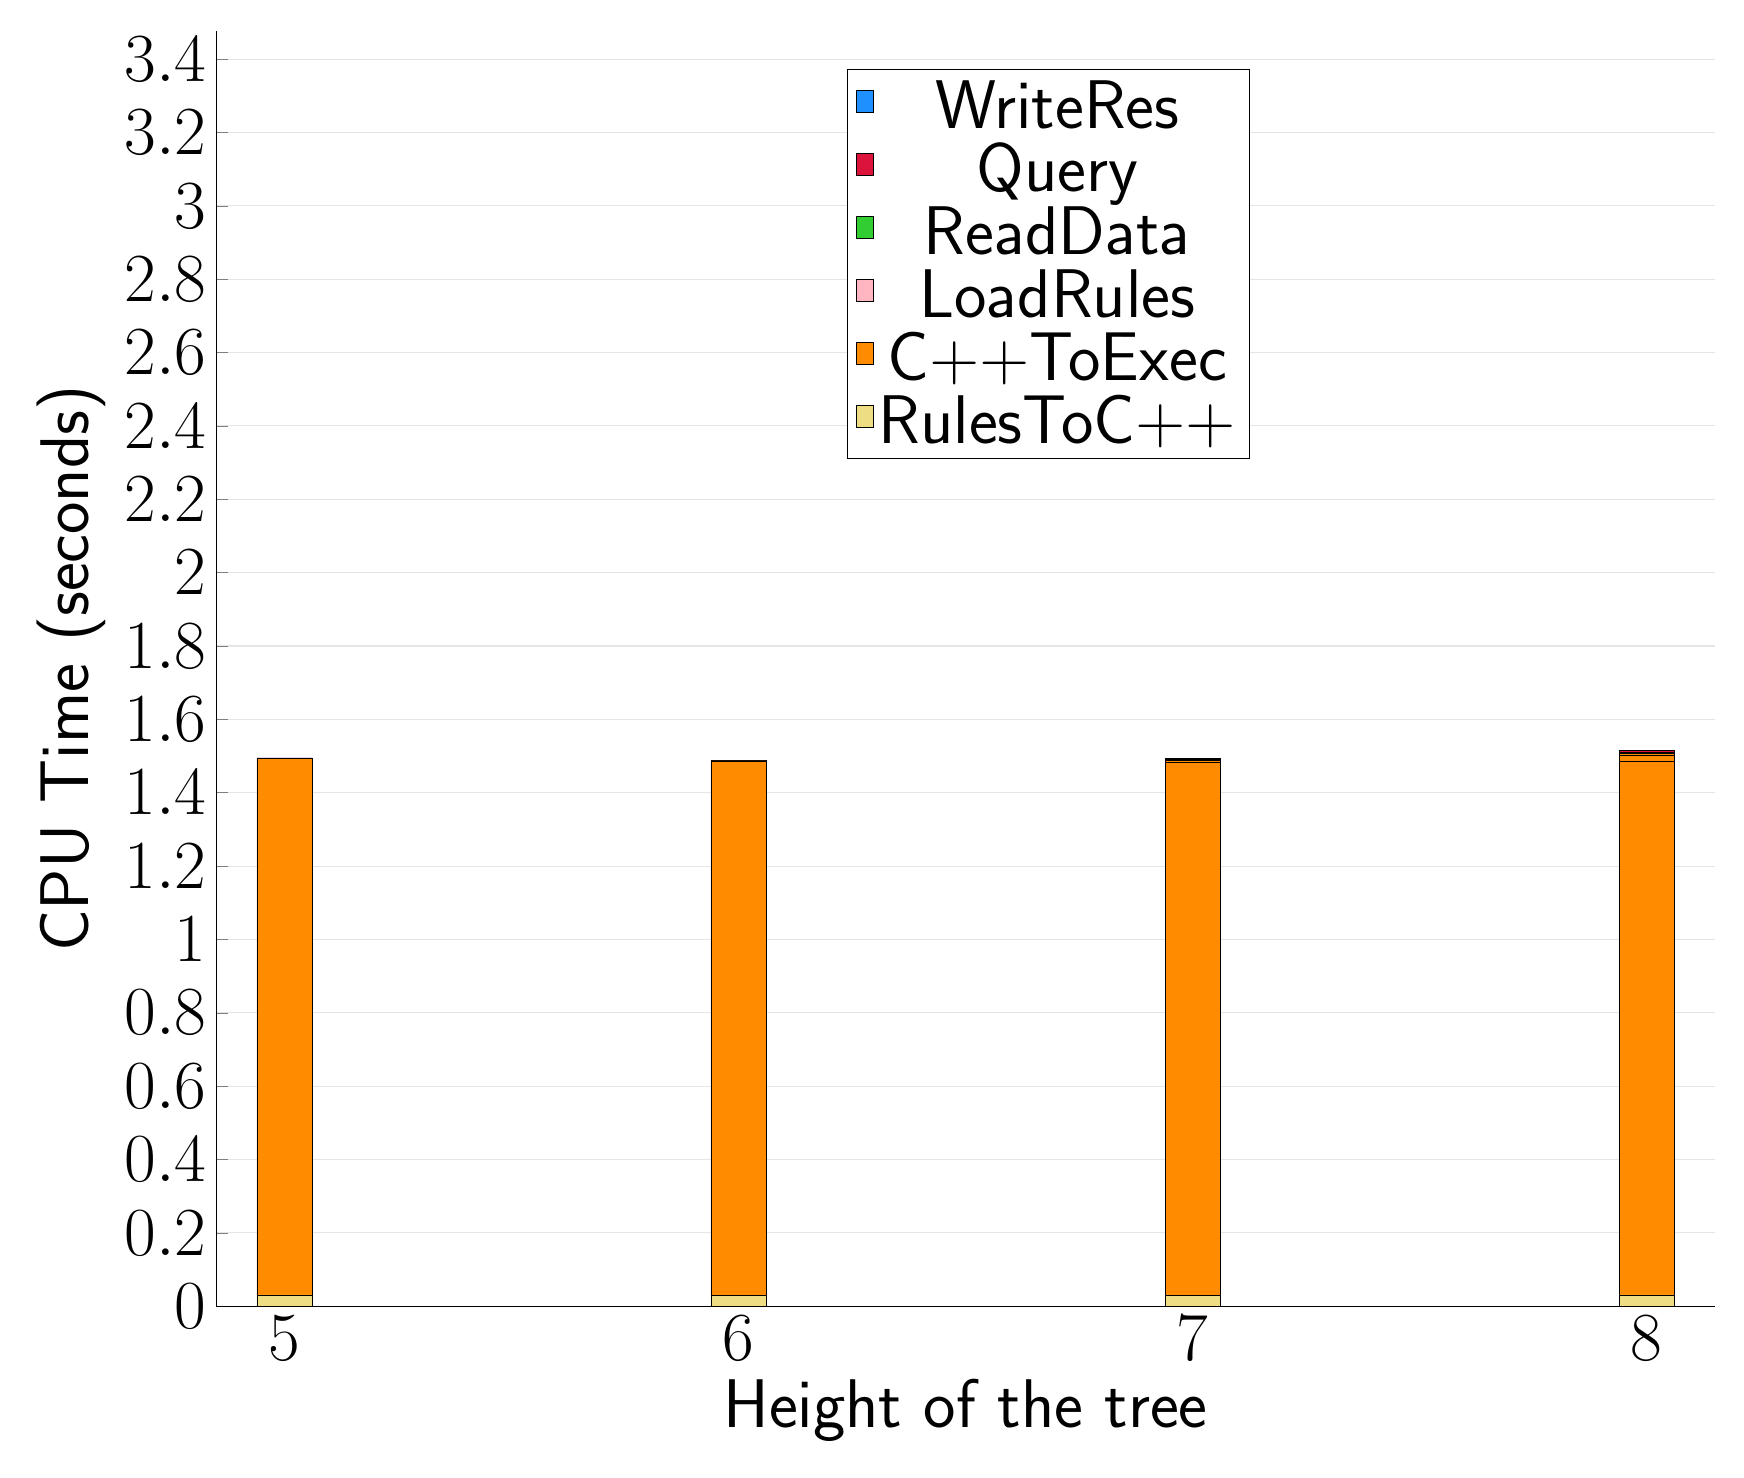
\begin{tikzpicture}
	\begin{axis}[
			ybar stacked,
			width=1.7\textwidth,
			bar width=0.7cm,
			ymajorgrids, tick align=inside,
			major grid style={draw=gray!20},
			xtick=data,
			ymin=0, ymax=3.477,
			axis x line*=bottom,
			axis y line*=left,
			enlarge x limits=0.05,
			legend style={
					at={(0.69, 0.97)},
					anchor=north east,
					legend columns=1,
					font=\Huge,
				},
			ylabel={CPU Time (seconds)},
			xlabel={Height of the tree},
			label style={font=\Huge},
			tick label style={font=\Huge},
		]
		\addlegendimage{fill=DodgerBlue, draw=black, line width=0.2pt}
		\addlegendentry{WriteRes}
		\addlegendimage{fill=Crimson, draw=black, line width=0.2pt}
		\addlegendentry{Query}
		\addlegendimage{fill=LimeGreen, draw=black, line width=0.2pt}
		\addlegendentry{ReadData}
		\addlegendimage{fill=LightPink, draw=black, line width=0.2pt}
		\addlegendentry{LoadRules}
		\addlegendimage{fill=DarkOrange, draw=black, line width=0.2pt}
		\addlegendentry{C++ToExec}
		\addlegendimage{fill=LightGoldenrod, draw=black, line width=0.2pt}
		\addlegendentry{RulesToC++}
		\addplot +[fill=LightGoldenrod, draw=black, line width=0.2pt] coordinates {
				(5, 0.031000000000000007)
				(6, 0.030000000000000006)
				(7, 0.030000000000000006)
				(7, 0.030000000000000006)
				(7, 0.030000000000000006)
				(8, 0.030999999999999993)
				(8, 0.031000000000000007)
				(8, 0.030000000000000006)
			};
		\addplot +[fill=DarkOrange, draw=black, line width=0.2pt] coordinates {
				(5, 1.4629999999999999)
				(6, 1.457)
				(7, 1.4580000000000002)
				(7, 1.4609999999999999)
				(7, 1.454)
				(8, 1.471)
				(8, 1.4769999999999999)
				(8, 1.4569999999999999)
			};
		\addplot +[fill=LightPink, draw=black, line width=0.2pt] coordinates {
				(5, 0.0001265)
				(6, 0.0001102)
				(7, 0.00011059999999999998)
				(7, 0.0001081)
				(7, 0.00011980000000000001)
				(8, 0.0001105)
				(8, 0.00012460000000000002)
				(8, 0.0001239)
			};
		\addplot +[fill=LimeGreen, draw=black, line width=0.2pt] coordinates {
				(5, 0.0003248)
				(6, 0.0003892)
				(7, 0.0005269000000000001)
				(7, 0.0005139)
				(7, 0.0005077)
				(8, 0.0007628)
				(8, 0.0008121000000000002)
				(8, 0.00081)
			};
		\addplot +[fill=Crimson, draw=black, line width=0.2pt] coordinates {
				(5, 0.0002724)
				(6, 0.0008173000000000002)
				(7, 0.0021675999999999996)
				(7, 0.0020836)
				(7, 0.0020743000000000003)
				(8, 0.0054711000000000004)
				(8, 0.005651700000000001)
				(8, 0.005616800000000001)
			};
		\addplot +[fill=DodgerBlue, draw=black, line width=0.2pt] coordinates {
				(5, 0.0002803)
				(6, 0.00034350000000000006)
				(7, 0.000501)
				(7, 0.0005005)
				(7, 0.0005020000000000001)
				(8, 0.0008337)
				(8, 0.0009297999999999999)
				(8, 0.0008827000000000002)
			};
	\end{axis}
\end{tikzpicture}

\end{document}
